\documentclass[usenames,dvipsnames,tikz]{standalone}
%\usetikzlibrary{shapes.geometric}
%\usepackage{rotating}
%\usepackage{xcolor}
%\definecolor{tLightOrange1}{HTML}{FFCD4F} %tikz color
%\colorlet{tLightGreen}{LimeGreen!70!OliveGreen!30!White}
%\colorlet{tBlue}{RoyalBlue!35!Cerulean}
%\colorlet{tRed}{Red}
%\definecolor{tLightGreen}{HTML}{D3ECAA}
%\colorlet{tLightOrange}{Dandelion!65!White}
%\definecolor{tLightPink}{HTML}{FFD4EB} %tikz color
%\definecolor{tLightBlue}{HTML}{CEF0FF} %tikz color

%\usepackage{tikz}
%\usepackage{standalone}
\begin{document}
	
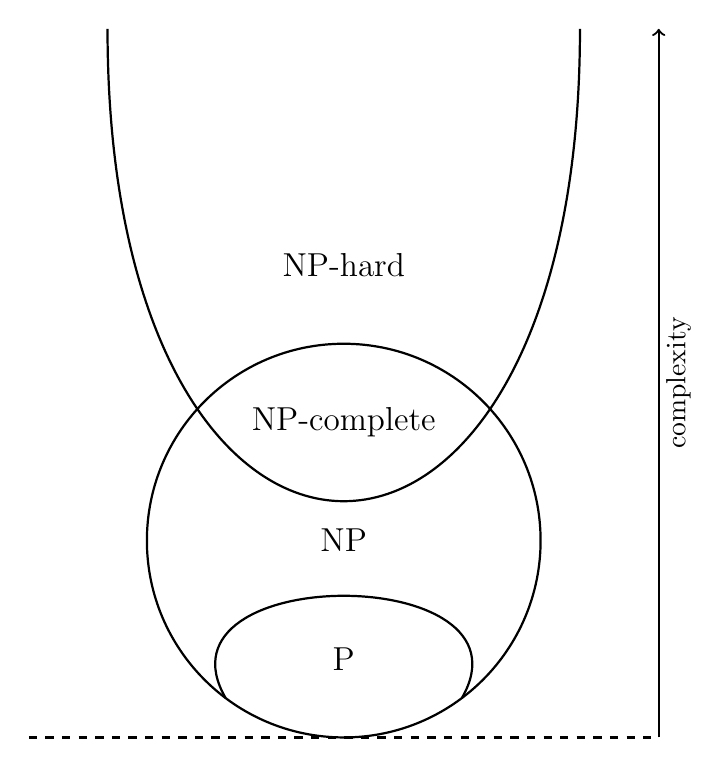
\begin{tikzpicture}

%\draw [help lines] (-1,-1) grid (9, 14);

%Vertical
\draw [thick,dashed] (0,0) -- (8,0);
\draw [thick, ->] (8,0) -- (8,9);
\draw [thick] (4,2.5) circle [radius = 2.5];
\node at (4,2.5) {\large NP};
\draw [thick] (2.5,0.5) to[out=120,in=60, distance=2cm] (5.5,0.5);
\node at (4,1) {\large P};
\draw [thick] (1,9) to[out=270, in=270, distance = 8cm] (7,9);
\node at (4,4) {\large NP-complete};
\node at (4,6) {\large NP-hard};

\node [rotate=90] at (8.25,4.5) {complexity};

%Horizontal
%\draw [thick,dashed] (0,0) -- (0,8);
%\draw [thick, ->] (0,0) -- (9,0);
%\draw [thick] (2.5,4) circle [radius = 2.5];
%\node at (2.5,5.5) {\Large NP};
%\draw [thick] (0.5,5.5) to[out=30,in=330, distance=2cm] (0.5,2.5);
%\draw [thick] (9,7) to[out=180, in=180, distance = 7.5cm] (9,1);





\end{tikzpicture}
	
\end{document}
